\section{Introduction}
Planetary anthropogenic threats are reshaping patterns of species diversity. Land-use change globally impact local species richness (\cite{Newbold2015}). In turn, species losses can negatively affect ecosystem functioning (\cite{Hooper2005}, \cite{Hooper2012}). Understanding how increasing pressures will affect ecosystem functioning and the services they provide is vital to put into place efficient mitigation measures.
   
The earliest experiments investigating the effect of species richness on the stability of ecosystem processes were conducted in the late twentieth century (\cite{Tilman1994}, \cite{Naeem1994}). Hundreds of grassplot experiments have since then confirmed that higher diversity promotes higher primary productivity and increased ecosystem stability (\cite{Tilman2014}). Intuitive mechanistic explanations of this phenomenon include increased niche complementary and resource partitioning, favouring more efficient resource use. Specifically, species properties (or traits) shape how species interact with their biological and physical environment. As such, species traits are central to elucidate how species diversity links to ecosystem functions. 

Strictly, traits are defined as phenotypic characteristics measurable the level of an individual, with an effect on organismal fitness or performance (\cite{McGill2006}, \cite{Violle2007}). They can be physiological (e.g., metabolic rates), morphological (e.g., body mass), behavioural (e.g., activity time), phenological (e.g., anthesis); they can also relate to species life-history (e.g., longevity) or diet (e.g, trophic level).
Traits shape species fundamental and realised niches; for instance, physiological traits influence species thermal tolerances, participating in defining their geographical distributions (\cite{Calosi2010}, \cite{Khaliq2017}). Morphological attributes (e. g. body mass, eye position...) participate in shaping the structure of food webs, and in determining the strength of inter- and intra-specific competition (\cite{Gravel2016}, \cite{Laigle2018}). As such, traits determine how species use and impact on their environment. Specifically, effect traits underpin species resource use and define organismal contributions to ecosystem functions. Response traits are those involved in determining species responses to environmental changes and can overlap with effect traits. This distinction between response and effect trait led to the development of a conceptual framework, the `response--effect' paradigm (\cite{Lavorel2002}, \cite{Luck2012}; see Chapter 1), which aims to understand how traits shape species responses to environmental changes, and how these changes in turn affect ecosystem functioning. 

A looser, more flexible definition of trait is sometimes adopted. Some characteristics only measurable at the species level can be referred to as `ecological' traits. Examples of ecological traits, only measurable in relation to species occurrence, include habitat preferences (breadth or thermal/moisture preferences). In this chapter, I use this more flexible definition of trait, and consider species `ecological' traits.

Trait-based approaches are increasingly used to understand processes underpinning species coexistence and biodiversity--ecosystem functioning relationships. Notably, their are widely employed in the context of the response--effect paradigm, and publications in this field have increased exponentially (\cite{Hevia2017}). Nevertheless, studies investigating how environmental changes are likely to affect species and ecosystem functions non-randomly with respect to species traits are both extremely taxonomically biased in favour of plants and invertebrates (more than 75\% of analysed studies in the metanalysis conducted by \cite{Hevia2017}), and spatially biased towards local scales (about 60\% of the studies in the metanalysis conducted by \cite{Hevia2017}; more than 90\% of the studies were conducted at local or national scales). Consequently, our understanding of biodiversity--ecosystem functioning relationships at various spatial scales need to be refined (\cite{Thompson2018}). Moreover, although terrestrial vertebrates have been extensively studied in the past (\cite{Titley2017}), how environmental changes may affect their global contributions to ecosystem functions needs to be investigated further. 

% finish referencing here
Indeed, vertebrates play diverse and important ecosystem roles. Through frugivory, they  contribute to seed dispersion (\cite{Wandrag2015}, \cite{Mokany2014}, \cite{McConkey2012}). They are significant pollinators in numerous ecosystems (\cite{Ratto2018}). They contribute in the regulation of animal and plant populations through predatory and herbivory activity (\cite{Luck2012}). As scavengers, they participate in nutrient cycling and energy transfers (\cite{Cunningham2018}, \cite{Inger2016}, \cite{Wilson2011}). Moreover, they are culturally important in many societies.

Understanding how environmental changes may affect their ecological roles is important to predict future ecosystem functioning, and to put into place appropriate mitigation measures. The end-goals of my PhD thesis include elucidating how species traits influence their responses to land-use and climate change at global scales, and how changes in community composition may affect ecosystem functions.

Addressing these questions requires to use extensive trait data. Despite vertebrates having been the focus of much research, and despite the growing interest for trait-based approaches, there exist no comprehensive database of vertebrate ecological traits encompassing all classes. Consequently, collating trait data was a prerequisite for any further work. This constituted the aim of this first chapter: here, I collected and imputed trait data across the four terrestrial vertebrate classes (mammals, birds, reptiles and amphibians).

In this chapter, I present the methods I used to collect and impute trait values across terrestrial vertebrates. Thanks to past and recent efforts to release data in the public domain, at least four comprehensive ecological trait databases are now freely accessible (mammals, PanTHERIA: \cite{Jones2009}; amphibians, AmphiBIO: \cite{Oliveira2017}; amniotes: \cite{Myhrvold2015}; both mammals and birds: \cite{Cooke2019}). Other trait datasets have been released on on-line platforms alongside published articles (e.g. Global Assessment of Reptile Distribution initiative, http://www.gardinitiative.org/), or can be downloaded from online databases (IUCN Red List (https://www.iucnredlist.org/), BirdLife data zone (http://datazone.birdlife.org/home). 

Data collection was constrained by the amount of information available in the literature.  All  primary sources offered a variety of traits, of which only a few were selected. Trait selection was motivated by two main reasons: (1) traits should be of ecological interest and be related to response or effect processes; (2) trait values should be available for many species, across the four terrestrial vertebrate classes, allowing for cross-classes comparative analyses. Targeted traits related to species life-history, morphology, behaviour and feeding habits (body mass; longevity; litter/clutch size; diel activity; trophic level; diet) and to their habitat preferences (habitat breadth and specialisation). Reptilian diet was not readily available in primary data sources, and one exception was made as I extracted diet data for the other classes. Species mobility was hardly available across sources, and no common variable could describe species mobility across classes. Although species' abilities to move in their environment is likely to strongly impact their responses to anthropogenic pressures, this trait was not considered for the above reasons. In this chapter, I detail the methodology I employed to collate targeted traits. I elaborate on some of the challenges met when compiling data across many species, such as inconsistency of taxonomy across sources, and problems posed by taxonomic inflation and synonymy.

Despite all the available primary sources, trait data was likely to be incomplete across terrestrial vertebrates. Many species were likely to present missing trait data for many traits; and taxonomic and geographical biases in the global trait knowledge were likely to exist (\cite{Hortal2014}). The gap in global trait knowledge was termed the `Raunki{\ae}r shortfall' by \cite{Hortal2014}. Here, I assessed the Raunki{\ae}r shortfall for terrestrial vertebrates. I investigated whether trait data presented taxonomic, phylogenetic and spatial biases. I also examined whether trait data presented systematic biases with regards to species conservation status. 

After examining patterns in the gaps in trait data information, I imputed missing trait values. This chapter finally details imputation methodology and examines imputation performance and robustness.

%In October 2018, Cooke et al released a comprehensive database of six mammalian and avian traits. They collated and imputed missing trait values for body mass, litter/clutch size, volancy, diel activity, primary diet and habitat breadth. As similar primary sources were used in both our data collection, I did not use their database to complement my sources. Moreover, the imputation methods they used to fill gaps in trait coverage differed from mine. I used this freely accessible compiled data as an opportunity to compare the results of both our data collection and imputation processes. Results of this comparison are available in the SI.


\section{Methods}

\subsection{Ecological trait data collection}

\subsubsection{Primary data sources.}
I collated ecological trait data for terrestrial vertebrates from the sources figuring in Table \ref{datasources}. Information was compiled for the following target traits: body mass, longevity, litter or clutch size, trophic level, diel activity, diet, and habitat preferences. I also compiled traits that were potentially correlated to either body mass or longevity, to be used as potential predictors in imputations of missing values. As such, body length information was compiled when available, as well as generation length or age at sexual maturity. Most notably, longevity was chosen over generation length or age at sexual maturity as it was the only common currency across classes reflecting generation turnover. In addition, species geographical range sizes were estimated from distribution data, extracted from the IUCN Red List.

% Table of sources.
\begin{table}[h!]
\renewcommand{\baselinestretch}{1}
\renewcommand{\arraystretch}{1.5}
\begin{center}\fontsize{9}{11}\selectfont
\caption[Primary sources used for each compiled trait.]{\textbf{Primary sources used for each compiled trait.} Primary sources may contain more traits than shown here. \textbf{BM}: body mass; \textbf{BL}: body length; \textbf{L}: longevity or maximum longevity; \textbf{GL}: generation length; \textbf{LCS}: litter or clutch size; \textbf{TL}: trophic level; \textbf{Di}: diet; \textbf{DA}: diel activity; \textbf{RS}: range size; \textbf{H}: habitat data. Bolded abbreviations highlight target traits; other traits were added for potential correlations in further imputations.} 
\label{datasources}
\begin{tabular}{|l|c|c|c|c|c|c|c|c|c|c|c|c|}
\hline
\multicolumn{1}{|c|}{\multirow{2}{*}{\textbf{Sources}}} & \multirow{2}{*}{\textbf{Taxa}} & \multicolumn{9}{c|}{\textbf{Traits}} & \multirow{2}{*}{\textbf{RS}} & \multirow{2}{*}{\textbf{H}} \\ \cline{3-11}
\multicolumn{1}{|c|}{} &  & \textbf{BM} & BL & \textbf{L} & MA & GL & \textbf{LCS} & \textbf{TL} & \textbf{Di} & \textbf{DA} &  &  \\ \hline
\cite{Oliveira2017} & \multirow{4}{*}{Amphibians} & \checkmark & \checkmark & \checkmark & \checkmark &  & \checkmark & \checkmark & \checkmark & \checkmark &  &  \\ \cline{1-1} \cline{3-13} 
Cooper &  &  & \checkmark &  &  &  & \checkmark &  &  &  & \checkmark &  \\ \cline{1-1} \cline{3-13} 
Senior &  &  & \checkmark &  &  &  &  &  &  &  &  &  \\ \cline{1-1} \cline{3-13} 
Bickford &  &  & \checkmark &  &  &  &  &  &  &  & \checkmark &  \\ \hline
\cite{Wilman2014} & \multirow{2}{*}{Birds} & \checkmark &  &  &  &  &  &  & \checkmark & \checkmark &  &  \\ \cline{1-1} \cline{3-13} 
Butchart &  & \checkmark &  &  &  & \checkmark &  &  &  &  &  &  \\ \hline
\cite{Jones2009} & \multirow{5}{*}{Mammals} & \checkmark & \checkmark & \checkmark & \checkmark &  & \checkmark &  &  & \checkmark &  &  \\ \cline{1-1} \cline{3-13} 
\cite{Kissling2014} &  &  &  &  &  &  &  & \checkmark &  &  &  &  \\ \cline{1-1} \cline{3-13} 
\cite{Gainsbury2018} &  &  &  &  &  &  &  & \checkmark &  &  &  &  \\ \cline{1-1} \cline{3-13} 
\cite{Wilman2014} &  & \checkmark &  &  &  &  &  &  & \checkmark & \checkmark &  &  \\ \cline{1-1} \cline{3-13} 
\cite{Pacifici2013} &  & \checkmark &  & \checkmark & \checkmark & \checkmark &  &  &  &  &  &  \\ \hline
\cite{Scharf2015} & \multirow{8}{*}{Reptiles} & \checkmark &  & \checkmark & \checkmark &  & \checkmark & \checkmark &  & \checkmark &  &  \\ \cline{1-1} \cline{3-13} 
%Meiri &  &  &  &  &  &  &  & \checkmark &  & \checkmark &  &  \\ \cline{1-1} \cline{3-13} 
\cite{Vidan2017} &  &  &  &  &  &  &  &  &  & \checkmark &  &  \\ \cline{1-1} \cline{3-13} 
\cite{Stark2018} &  & \checkmark &  & \checkmark &  &  & \checkmark &  &  & \checkmark &  &  \\ \cline{1-1} \cline{3-13} 
\cite{Schwarz2017} &  &  &  &  &  &  & \checkmark &  &  &  &  &  \\ \cline{1-1} \cline{3-13} 
\cite{Novosolov2017} &  & \checkmark &  &  &  &  &  & \checkmark &  &  & \checkmark &  \\ \cline{1-1} \cline{3-13} 
\cite{Novosolov2013} &  &  &  &  &  &  & \checkmark &  &  &  &  &  \\ \cline{1-1} \cline{3-13} 
\cite{Slavenko2016} &  & \checkmark &  &  &  &  &  &  &  &  &  &  \\ \hline
\cite{Myhrvold2015} & Amniotes & \checkmark & \checkmark & \checkmark & \checkmark &  & \checkmark &  &  &  &  &  \\ \hline
IUCN & Vertebrates &  &  &  &  &  &  &  &  &  & \checkmark & \checkmark \\ \hline
\end{tabular}
\end{center}
\end{table}

\subsubsection{Compilation methods.}

\paragraph{Continuous traits.}
All continuous traits were averaged within species when different sources provided estimates. Longevity and maximum longevity were assumed to provide the same information and were averaged within species. No measure of intra-specific variability was compiled and estimates were provided as a single measure for each species.

\paragraph{Categorical traits.}
\subparagraph{Activity time.}
Species were described as being either nocturnal or non-nocturnal. Despite a higher resolution of activity time information in some of the primary sources (e.g. species being described as cathemereal, crepuscular or strictly diurnal), I adopted the classification of the primary source with the lowest resolution, in order to have consistent information across classes.
\subparagraph{Diet and diet breadth.}
For mammals and birds, diet was compiled from the Elton Traits database (ref). Primary diet was available in the avian dataset and declined into five categories: (1) plant or seed consumers; (2) fruit or nectar consumers; (3) vertebrate consumers, including fish and carrion; (4) invertebrate consumers; and (5) omnivores. Primary diet was not available for mammals. Instead, mammal diet was only described as the percent use of different food items. I pooled these items together into the same five primary diet categories as for the avian dataset. Any food items for which percent use was equal to or above 50\% were considered to be primary food items. Species for which no food item had percent use above 50\% were considered to be omnivores.\\ 
For amphibians, diet information was extracted from AmphiBIO. Diet information was available as binary variables for diverse food items. Percent use were not recorded, so these items were considered to form species primary diet. I pooled amphibian species into the five diet categories described above.
\subparagraph{Trophic level.} For amphibians and birds, trophic levels were partly inferred from the primary diet. 
\subparagraph{Habitat preferences.}
Species habitat preferences were compiled from IUCN habitat data files and were described as a binary variable recording whether a species was known to occur in a particular habitat. I calculated habitat breadth as the number of habitats a species was known to use. Weights were assigned to each habitat in this calculation depending on the recorded habitat suitability and importance; outcomes were not very sensitive to the presence of weights (compared to a non-weighted sum, see SI). Finally, a broad degree of habitat specialisation was produced. If any artificial habitat was recorded to be suitable, species were reported to be generalists; else, they were natural habitat specialists. More details on habitat preferences compilation are provided in the SI. 

\subsection{Phylogenetic information}
I obtained phylogenetic trees for birds, amphibians, mammals and squamates from Hedges et al (2015) (available at \url{http://www.biodiversitycenter.org/ttol}, downloaded 06/07/2018). All trees were ultrametric and fully resolved, except for the amphibian tree which presented polytomies. All trees contained a few branches of length 0 (193 branches for mammals, 136 for amphibians, 189 for birds and 284 for reptiles).

\subsection{Tackling taxonomic synonymy}
Across the different primary sources, similar species could appear under different binomial names. This was a problem when matching datasets by species. It was also problem when matching species to the PREDICTS database. Moreover, it is possible than within a primary source, a given species was appearing under two or more different names. As such, taxonomic synonymy created `pseudoreplicates' of the same species, overall falsely increasing the total number of species and artificially inflating the amount of missing trait values. Taxonomic synonymy was hence a major issue; due to the large number of species across datasets, extensive manual checks could not be applied. The presence of typos in species names had the same effect as synonymy, erroneously duplicating species. I attempted to correct for taxonomy first by correcting for typos, and second by identifying species which were entered under a synonymic name and replacing these with the accepted name. To this end, I developed an automated procedure, complemented with a few manual entries. Obvious cases where vernacular names had been entered in the place of binomial names were also treated manually; that was the case for 44 PREDICTS species (when possible, I best assigned binomial names to species common names; unidentifiable species were left empty and assigned to a genus (5 species)).

\subsubsection{Automated procedure and outputs.}
\paragraph{Extracting names from the IUCN Red List and the Integrated Taxonomic Information System (ITIS).}
The automated procedure consisted in extracting species accepted and synonymic binomial names from the IUCN Red List or from the ITIS, using the rredlist and taxize R packages. I started by generating a list of all names figuring across datasets (primary sources, phylogenies and PREDICTS). These `original' names were corrected for typos; then, the IUCN Red List was queried and synonyms and accepted names were stored when possible. When species were not found in the IUCN Red List, information was extracted from ITIS. When species were not found in ITIS either, corrected names were assumed to be accepted. Family and order information was extracted using the same procedure and some entries were completed using the Global Biodiversity Information Facility taxonomic backbone (\url{https://www.gbif.org/tools/species-lookup}).\\
\textbf{NB:} for species entered with the forms \textit{Genus cf.}, \textit{Genus aff.} or \textit{Genus spp.}, the accepted name was left empty.

\paragraph{Outputs.} I generated a list of vertebrate species, recording whether species names were accepted or synonymic (for 14124, 8743, 6090, and 11183 names or identifiers found across datasets for birds, amphibians, mammals and reptiles respectively, including species names as they appeared in phylogenetic trees). For each name, the identified accepted name and the synonyms were stored when possible, as well as additional taxonomic information (order, family, genus). When queries did not succeed, species accepted names were assumed to be the original names found in the datasets.

\paragraph{Harmonising taxonomy in trait datasets.}
Taxonomy across datasets was finally homogenised by replacing recorded synonyms with their accepted scientific names. Overall, this procedure  reduced the total number of species figuring in trait datasets (Figure \ref{taxcor}). The species presenting the highest degree of pseudoreplication was the East African mole rat (\textit{Tachyoryctes splendens}), which was figuring under 12 names identified as being synonymic across primary sources (Figure \ref{taxcor}B), highlighting the need for normalising taxonomy across sources.

% figure: distribution of names and differences in species number
\vspace{0.5cm}
\begin{figure}[h!]
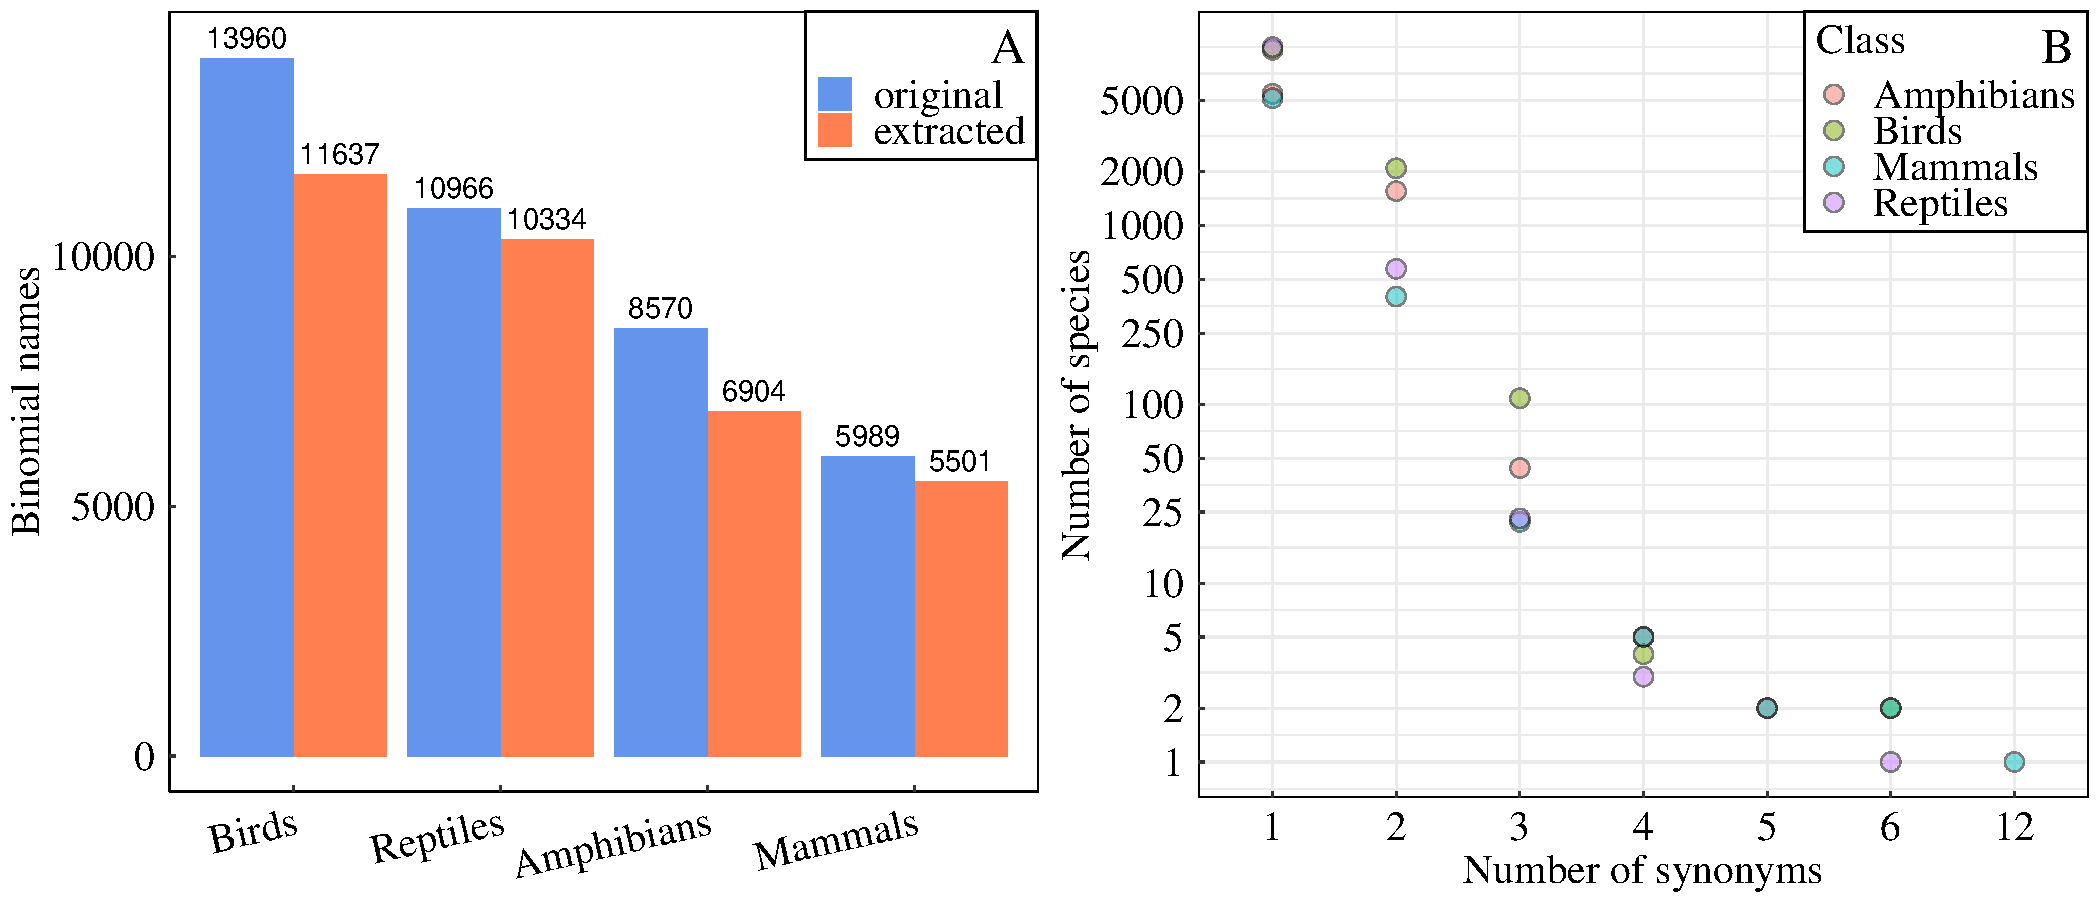
\includegraphics[scale=0.45]{figures/chapter2/Taxonomic_corrections/tax_corrections}
\caption[Difference in species number due to taxonomic correction (A) and distribution of number of synonyms across datasets (B)]{\textbf{Difference in species number due to taxonomic correction (A) and distribution of number of synonyms across datasets (B).} \textbf{(A)} shows the number of species across all primary sources (trait datasets and PREDICTS, excluding phylogenies), before and after correcting for taxonomy. Replacing identified synonyms by the extracted accepted name reduced the number of species in all classes, with the most drastic reduction for birds (decrease by 2,323 unique binomial names). The diminution was of 632 unique identified species for reptiles, of 1,666 for amphibians and of 488 for mammals. \textbf{(B)} shows the distribution of the number of synonymic names. In all four classes, more than 5,000 species (or binomial names) had no identified synonyms. Nevertheless, a large amount of species had two identified synonyms (range: 400 species for mammals - 2086 for birds). The most replicated species was the East African mole rat \textit{Tachyoryctes splendens}, for which 11 synonyms were identified.}
\label{taxcor}
\end{figure}

Despite the automation efforts, taxonomic redundancy persisted to a degree in the trait datasets. Indeed, at this stage, not all species in PREDICTS matched a species in the trait datasets. Additional manual inputs were required to resolve taxonomic synonymy for these species. Verifying the presence of PREDICTS species in trait datasets was important for further analyses. Taxonomic synonymy was resolved manually for 91 PREDICTS species that did not match any species in the trait datasets; in that case, information was extracted from other diverse sources (such as the Reptile Database (\url{http://www.reptile-database.org/}); Avibase (\url{https://avibase.bsc-eoc.org/avibase.jsp?lang=EN&pg=home}); AmphibiaWeb (\url{https://amphibiaweb.org/})). After adding manual inputs to the synonym datasets, all PREDICTS species were represented in trait datasets. 

The need to apply additional manual inputs underlines the fact that the automated procedure was not optimal. The Red List and the ITIS were not comprehensive taxonomic sources, and for clades with high degrees of pseudoreplication in names, such as reptiles or amphibians, neither the Red List or the ITIS were fully resolved. As I only applied manual checks for PREDICTS relevant species, `pseudoreplication' and taxonomic errors are likely to have persisted to a degree. Moreover, certain species were entered using the format \textit{Genus subspecies} rather than \textit{Genus species}; for these, automated queries may have failed to identify the species.

% Extract of synonym dataset? in the SI


\subsubsection{Harmonising taxonomy in phylogenetic trees and increasing species phylogenetic representation.}

\paragraph{Taxonomic correction across tip labels.} 
Efforts to correct datasets for taxonomy created problems for a marginal proportion of species when dealing with phylogenies. The idea of the procedure described above was to replace two or more identified synonyms by a single accepted name, and then collapsing dataset rows together by names. I applied the same method on phylogenies, replacing synonyms by their identified accepted names in trees' tip labels. Not unexpectedly, in some cases, the procedure ended up assigning the same accepted name to different phylogenetic tips. This was the case for 2.8\% of mammalian, 1.7\% of avian, 1.6\% of amphibian and  1.7\% of reptilian species, which then had multiple phylogenetic positions (most having two different positions, see SI). Because keeping several putative phylogenetic positions for a species was problematic in further analyses, I selected one tip to conserve and dropped other tips from the phylogenies (Figure \ref{chart_phylorep}). To briefly describe the procedure, if replicated tips were sister clades, the tip to conserve was chosen randomly among the replicates. Else, I chose to conserve the tree tip whose position was closest to the position of the same tip in the uncorrected tree, when present. In all other few cases, tips to drop were chosen randomly. Further details on how replicated tips were dropped are available in the SI (with 3 examples for each case of Figure \ref{chart_phylorep}).

\begin{figure}[h!]
\centering
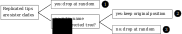
\includegraphics[scale=0.7]{figures/chapter2/chart_phylorep}
\caption[Procedure followed to drop replicated tips from phylogenies]{\textbf{Procedure followed to drop replicated tips from phylogenies.} Most of these were replicated twice. When replicated tips were sister clades, the tips to drop were chosen randomly, as it did not affect the `true' phylogenetic position of the species (1). When replicated were not sister clades, I kept the tip whose position was closest to the position of the same tip in the uncorrected tree (2). In a few cases, the corrected name did not appear in the original tree. Those were problematic cases, and the tips to drop were chosen randomly (3). Nevertheless, occurences of that third case were rare (see SI).}
\label{chart_phylorep}
\end{figure}

\begin{figure}[h!]
\centering
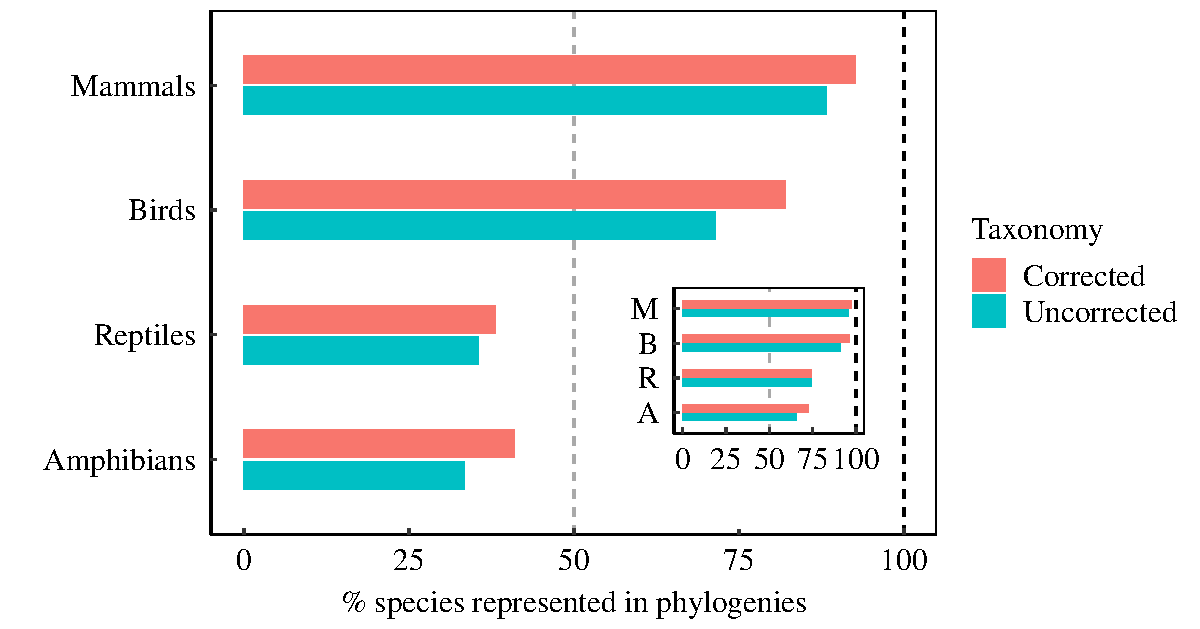
\includegraphics[scale=0.7]{figures/chapter2/Species_representation_phylo}
\caption[Percentage of species represented in the phylogenies for both corrected and uncorrected trait datasets]{\textbf{Percentage of species represented in the phylogenies for both corrected and uncorrected trait datasets.} Overall, taxonomic correction increased species representation in phylogenetic trees. Representation for mammals and birds was high (after taxonomic correction: 82\% of avian and 93\% of mammalian species had a phylogenetic position). On the other hand, reptiles and amphibians were poorly represented (after taxonomic correction: only 38\% of reptilian and 41\% of amphibian species were placed in phylogenetic trees). The inset barplot shows representation for species figuring in PREDICTS. For these, species presence in phylogenetic trees after correction was high across all classes, with a minimum representation of 76\% for amphibians.}
\label{species_rep_phylo}
\end{figure}

\paragraph{Correcting for taxonomy in the phylogenies: conclusions.}
Overall, correcting for taxonomy in phylogenies improved species representation in the trees (Figure \ref{species_rep_phylo}. For amphibian and reptilian species figuring in PREDICTS only, phylogenetic representation disproportionally increased (with a minimum representation of 76\% for PREDICTS amphibians after correcting the trees for taxonomy, inset plot in Figure \ref{species_rep_phylo}). Nevertheless, correcting phylogenetic tip labels generated replicates for a marginal number of tips, which then had to be dropped. 


\paragraph{Species attachments to phylogenetic trees.} Some species in the trait datasets were not represented in the phylogenies. Maximising the number of species represented in the phylogenies was important for further trait imputations. Indeed, if traits were evolutionary conserved, species phylogenetic position could be an important predictor of trait values. To maximise species representation, I added some species to the root of their genus, when possible (phytools package). Attaching species at the root of their genus created polytomies, which were resolved randomly (using multi2di and bifurcatr, ape and PDcalc packages). Resulting trees contained additional branches of length zero. Such modifications of the phylogenetic trees could have altered the significance and the strength of trait phylogenetic signal. I further verify whether these alterations of the trees had impacted phylogenetic signal, by qualitatively comparing the strength and the significance of phylogenetic signal for each trait, estimated using both original trees and augmented trees (see `Assessing phylogenetic signal in traits').

Finally, a large number of species were attached to their genus in the trees (Table \ref{random_attachments_phy}). For instance, only 38\% of the species figuring in the reptilian trait dataset were initially found in the squamate phylogeny. After attaching non-represented species, 91\% of the species were placed in the squamate phylogeny. 

\begin{table}[h!]
\renewcommand{\baselinestretch}{1}
\renewcommand{\arraystretch}{1.5}
\begin{center}\fontsize{9}{11}\selectfont
\caption[Species representation in phylogenetic trees (corrected taxonomy)]{\textbf{Species representation in phylogenetic trees (corrected for taxonomy).} The number of species attached to the root of their genus ranged from 175 (mammals) to 5438 (reptiles). Finally, most species were represented in the phylogenies, whereas more than half reptilian and amphibian species initially had no known phylogenetic position.} 
\label{random_attachments_phy}
\begin{tabular}{|l|l|l|c|l}
\cline{1-4}
\multicolumn{1}{|c|}{\textbf{Class}} & \multicolumn{1}{c|}{\textbf{Initially not in tree}} & \multicolumn{1}{c|}{\textbf{Of which randomly attached}} & \textbf{No final representation in tree} &  \\ \cline{1-4}
Amphibians                  & 59\% (4040 of 6904)                           & 96\% (3883 of 4040)                     & \textbf{2.3\%}             &  \\ \cline{1-4}
Birds                       & 18\% (2085 of 11637)                          & 75\% (1574 of 2085)                    & \textbf{4.4\%}             &  \\ \cline{1-4}
Mammals                     & 7.4\% (407 of 5502)                           & 43\% (175 of 407)                       & \textbf{4.2\%}            &  \\ \cline{1-4}
Reptiles                    & 62\% (6391 of 10334)                          & 85\% (5438 of 6391)                    & \textbf{9.2\%}             &  \\ \cline{1-4}
\end{tabular}
\end{center}
\end{table}


\subsection{Exploring biases in the coverage and completeness of trait information across classes}
Having normalised taxonomy and compiled trait data, I assessed trait coverage, defined as the percentage of species for which trait information was available for a given trait. I also estimated the amount of trait information available for a species by calculating trait completeness. For a species, trait completeness was defined as the proportion of traits for which information was available (number of non-missing trait values divided by total number of traits). In corrected datasets, species with 0\% completeness in predictor traits were filtered out.

Further, I examined whether patterns in the distribution of missing values emerged within classes, as particular clades or parts of the phylogenies could be under-sampled compared to other clades.
Whether values are missing at random is likely to impact imputation errors, notably if some taxa appear to be under-sampled. To assess whether missing values presented patterns, I represented within-family median completeness and coverage values in each branch of phylogenetic trees built at the family level. Tree branches were colour-coded to reflect median values in each family. Specifically, within-family trait completeness was calculated by aggregating species into their families and calculating the median trait completeness within each group. 

Patterns of missing values in trait coverage were explored for each trait separately. Trait coverage was assessed within families as the number of species for which values were missing over the total number of species in each family. As families represented by very few species might present higher percentages of missing values, reflecting family size rather than randomness in sampling, I contrasted trait coverage plots against a plot showing how much each family contributed to the total number of species (number of species in each family over total number of species in the tree).

Trait coverage was highly variable across classes and traits (see Results). Trait coverage for species figuring in the PREDICTS database only overall improved compared to trait coverage for the whole set of species, particularly for reptiles and amphibians (see SI). Nevertheless, no trait reached 100\% coverage in any class. Obtaining trait estimates for all of PREDICTS species was important, as otherwise, each species for which trait values were missing would have to be dropped in further analyses. Moreover, within-class biases in availability of trait information appeared (see Results). Consequently, dropping missing-value species could skew trait distributions and generate biases in further analyses. As such, rather than dropping missing-value species, I aimed to fill coverage gaps by imputing missing trait values. 

\subsection{Imputing missing trait values}
In order to achieve full coverage across classes, I imputed missing trait values. Diverse imputation methods have been developed and used in published articles. Penone et al (2014) assessed the performance of four different imputation approaches (K-nearest neighbour (kNN, Troyanskaya 2001), multivariate imputation by chained equations (mice, van Buuren 2009, 2011), random forest algorithms as implemented in R by missForest (Stekhoven, 2011) and phylogenetic imputations implemented with phylopars (Goolsby, 2016)). Their study showed that the kNN approach resulted in significantly higher imputation error rates than the three other approaches. Both missForest and phylopars were the best methods when phylogenetic information was included. Nevertheless, phylopars was much slower than missForest, and could only handle continuous traits. missForest was faster and could deal with mixed type data. Without phylogenetic information, mice was found to be the best method, with fast imputations of mixed-type data. Of all these methods, missForest was the only one that did not make assumptions about data distribution (being a non-parametric approach), or that did not require a prior knowledge of some tuning parameters. As such, missForest appeared to be a robust option for missing data imputation. To further assess whether to use random forests rather than multivariate chained equations, I estimated the amount of phylogenetic signal in traits. Strong phylogenetic signal in traits would indicate than missForest could perform better than mice.

\subsubsection{Assessing phylogenetic signal in traits}

\paragraph{Measuring phylogenetic signal in continuous traits with Pagel's $\lambda$.}
Phylogenetic signal is a measure of the tendency of closely related species to resemble each other more than less related species. Diverse statistics have been developed to estimate phylogenetic signal, most of them applying to continuous traits (Munkemuller 2012). Here, I used Pagel's $\lambda$, estimated with the R function phylosig (phytools package), to assess the amount of phylogenetic signal in continuous traits. Pagel's $\lambda$ is a scaling component that measures the transformation that should be applied to the phylogenetic tree for a trait to have evolved under a pure Brownian motion model of evolution. Under a Brownian motion model of evolution, changes in trait values happen at random along the branches and trait variance is proportional to evolutionary time.  $\lambda$ is then close to zero: the trait covariance matrix is scaled down and the tree loses its internal structure. When $\lambda$ equals one, both the phylogeny and the trait covariance matrix remain unchanged and the structure of the tree explains trait evolution. As such, $\lambda$ values close to one indicate that trait values are more similar in closer related species.  

Using Pagel's $\lambda$, I assessed the strength of the phylogenetic signal. The phylosig function (phytools) also allows to test for signal significance (comparing the estimated $\lambda$ to the null expectation of $\lambda$ with a log-likelihood ratio test). 

\paragraph{Measuring phylogenetic signal in categorical traits with $\delta$ (Borges et al, 2018).}
Very few methods have been developed to measure and test phylogenetic signal in categorical traits. Fritz and Purvis (2010) introduced the $D$-statistic; nevertheless, $D$ is based on a discretisation of categorical traits, which reduces them to binary variables. Borges et al (2018) introduced a new statistic, called $\delta$, to measure phylogenetic signal in categorical traits of all types. Their approach uses Bayesian inferences to reconstruct trait evolution, that is, to infer trait values in ancestral nodes of the phylogeny. The underlying idea is that the  better the phylogeny explains trait evolution, the lower the uncertainty is in ancestral state inferences. As such, $\delta$ relies on the quantification of the uncertainty associated with the reconstruction of ancestral states. $\delta$ can take any positive number, with higher values indicating stronger signal. To test for the significance of the signal, the authors propose to compare the estimated value of $\delta$ with the null expectation  of $\delta$. 

I estimated phylogenetic signal in categorical traits with the $\delta$ statistic; implementation used the R code provided by Borges et al. To test for the significance of the signal, I generated null distributions of $\delta$  for each trait by randomising trait vectors 50 times (simulating Brownian motion model of trait evolution), and calculating $\delta$ for each randomised vector. I then calculated the median of simulated $\delta$ values as well as 95\% confidence intervals. I tested whether the null-medians were significantly lower than the observed value of $\delta$ using one-sided Wilcoxon rank sum tests. Note that the function developed by Borges et al cannot be implemented if phylogenetic trees contain branches of length 0. As both original and corrected phylogenies contained 0-length branches, I added a very small number to these ($10^{-10}$) to remedy to this issue and to test for phylogenetic signal. 

\paragraph{Significant phylogenetic signal in all traits}
All traits showed significant phylogenetic signal (Table \ref{physignal} and SI for p-values of statistical tests), although the strength of the signal was variable across classes and traits. Overall, modifying the original phylogenies by correcting for taxonomy and by attaching species to the root of their genus did not, qualitatively, have a strong impact on the signal (Figures \ref{signalcontinuous} and \ref{signalcategorical}), although differences were bigger in reptiles and amphibians, where more than 80\% of missing species were added to phylogenetic trees. In mammals and birds, phylogenetic signals remained similar. On the other hand,the stronger effects were observed for reptilian body mass, where adding species to the tree lowered the strength of the signal, and for amphibian trophic level, were the opposite was observed.

Phylogenetic signals in categorical traits were all highly significant (Figure \ref{signalcategorical}; p-values for Wilcoxon signed rank test: see SI). The strength of the signal differed across classes and traits, with diel activity, trophic level and primary diet showing particularly strong signal in mammals and birds. Reptiles also showed strong signals for diel activity and trophic level. For amphibians, the results were more even across traits, and still highly significant. Overall, the signal for habitat specialisation was less strong.

Most mammalian continuous traits had very strong phylogenetic signal ($\lambda \geq 0.9$), except habitat breadth ($\lambda \approx 0.7$). In birds, both habitat and diet breadth showed weaker signal, but other continuous traits were highly conserved across closely related species . For amphibians and reptiles, signal strength was much more variable, which may be due to poorer initial trait coverage across phylogenetic tips (see Results). Nevertheless, body length showed high signal in both these classes ($\lambda \geq 0.9$). 

\pagebreak

\begin{table}[h!]
\renewcommand{\baselinestretch}{1}
\renewcommand{\arraystretch}{1.5}
\begin{center}\fontsize{9}{11}\selectfont
\caption[Phylogenetic signal in continuous and categorical traits and in range size]{\textbf{Phylogenetic signal in continuous and categorical traits and in range size.} \textbf{BM}: body mass; \textbf{L}: longevity; \textbf{LCS}: litter/clutch size; \textbf{HB}: habitat breadth; \textbf{DB}: diet breadth; \textbf{GL}: generation length; \textbf{BL}: body length; \textbf{SM}: sexual maturity; \textbf{RS}: range size; \textbf{TL}: trophic level; \textbf{PD}: primary diet; \textbf{DA}: diel activity; \textbf{Sp}: specialisation. The phylogenetic signal in continuous traits was calculated with Pagel's $\lambda$. For categorical traits, the $\delta$ metric developed by Borges et al (2018) was used. A star indicates a significant signal (significant p-values scores for the log-likelihood ratio test in the case of $\lambda$; and significant difference from the simulated null distribution of $\delta$ for categorical traits, see SI). `na' are introduced for traits that were not considered in a class but may have been used in another as a predictor in missing values imputations. All traits showed significant phylogenetic signal, with signals for BM, L, LCS, and GL being particularly strong in mammals and birds (above 0.9). Here all calculations were conducted with the corrected phylogenies, after species additions at the root of their genus. See SI for phylogenetic signals computed with the original phylogenies.} 
\label{physignal}
\begin{tabular}{|l|c|c|c|c|c|c|c|c|c|c|c|c|c|}
\hline
\multicolumn{1}{|c|}{\multirow{2}{*}{\textbf{Class}}} & \multicolumn{9}{c|}{\textbf{\begin{tabular}[c]{@{}c@{}}Continuous target traits,\\ additional predictors and range size: $\lambda$\end{tabular}}} & \multicolumn{4}{c|}{\textbf{\begin{tabular}[c]{@{}c@{}}Categorical traits:\\ $\delta$\end{tabular}}} \\ \cline{2-14} 
\multicolumn{1}{|c|}{}                                & \textbf{BM}    & \textbf{L}   & \textbf{LCS}   & \textbf{HB}   & \textbf{DB}   & \textbf{GL}   & \textbf{BL}   & \textbf{SM}   & \textbf{RS}   & \textbf{TL}           & \textbf{PD}           & \textbf{DA}                & \textbf{Sp}          \\ \hline
\textbf{Mammals}                                      & 1.0*           & 0.97*        & 0.96*          & 0.70*         & 0.99*         & 0.99*         & 1.0*          & na            & 0.99*         & 17*                   & 50*                   & 19*                        & 1.4*                 \\ \hline
\textbf{Birds}                                        & 1.0*           & 0.87*        & 0.92*          & 0.50*         & 0.49*         & 0.99*         & na            & na            & 0.67*         & 10*                   & 18*                   & 28$\cdot$10$^3$*           & 1.6*                 \\ \hline
\textbf{Reptiles}                                     & 0.36*          & 0.81*        & 0.72*          & 0.39*         & na            & na            & 0.98*         & 0.87*         & 0.41*         & 4.3*                  & na                    & 7.1*                       & 1.5*                 \\ \hline
\textbf{Amphibians}                                   & 0.80*          & 0.33*        & 0.63*          & 0.77*         & 0.71*         & na            & 0.96*         & na            & 0.54*         & 18*                   & 3.7*                  & 2.9*                       & 3.6*                 \\ \hline
\end{tabular}
\end{center}
\end{table}

\begin{figure}[h!]
\centering
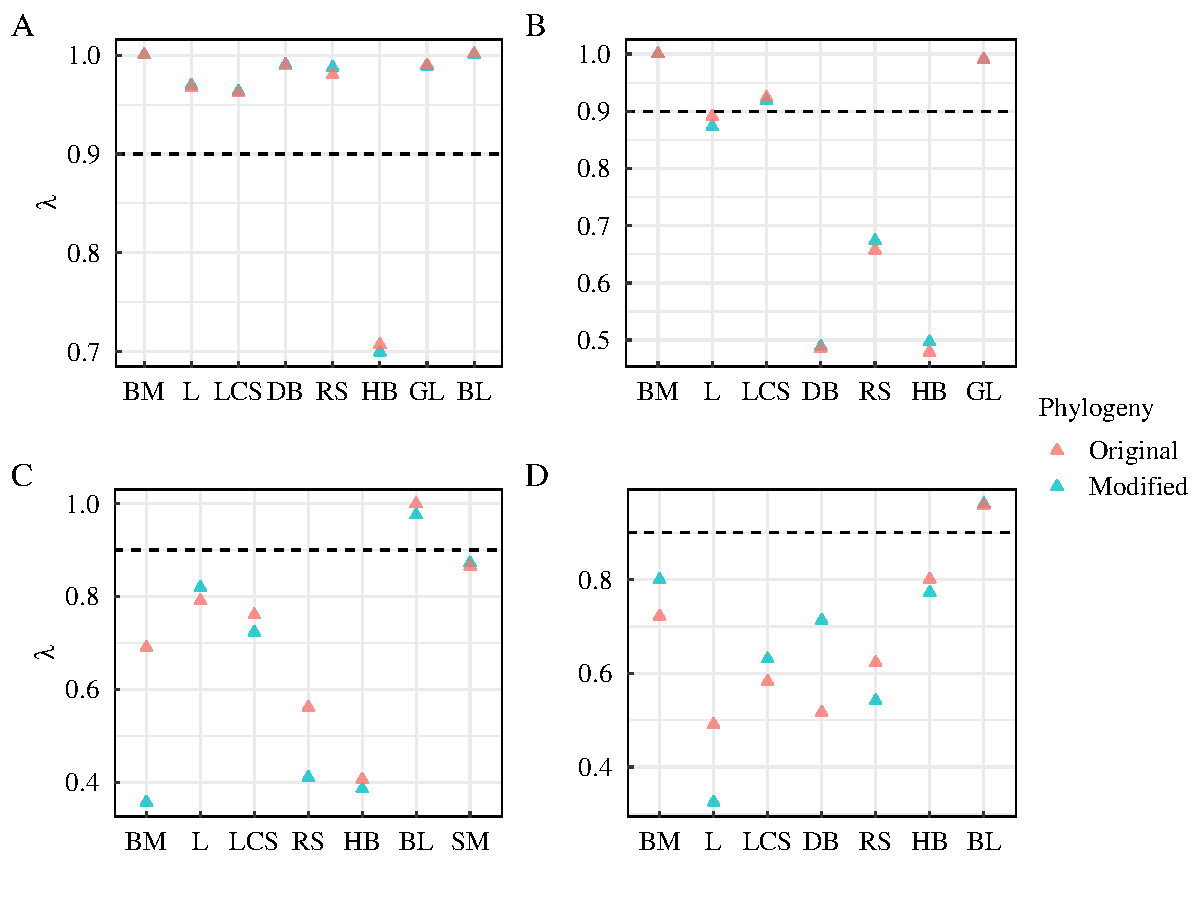
\includegraphics[scale=0.7]{figures/chapter2/Phylosignal/Continuous}
\caption[Phylogenetic signal in continuous traits (Pagel's $\lambda$) estimated with both original phylogenies and modified phylogenies]{\textbf{Phylogenetic signal in continuous traits (Pagel's $\lambda$) estimated with both original phylogenies and modified phylogenies.} \textbf{(A)} Mammals; \textbf{(B)} birds; \textbf{(C)} reptiles and \textbf{(D)} amphibians. Overall, altering the phylogenies by correcting for taxonomy and by increasing species representation did not have an important effect on $\lambda$.}
\label{signalcontinuous}
\end{figure}

\pagebreak

\begin{figure}[h!]
\centering
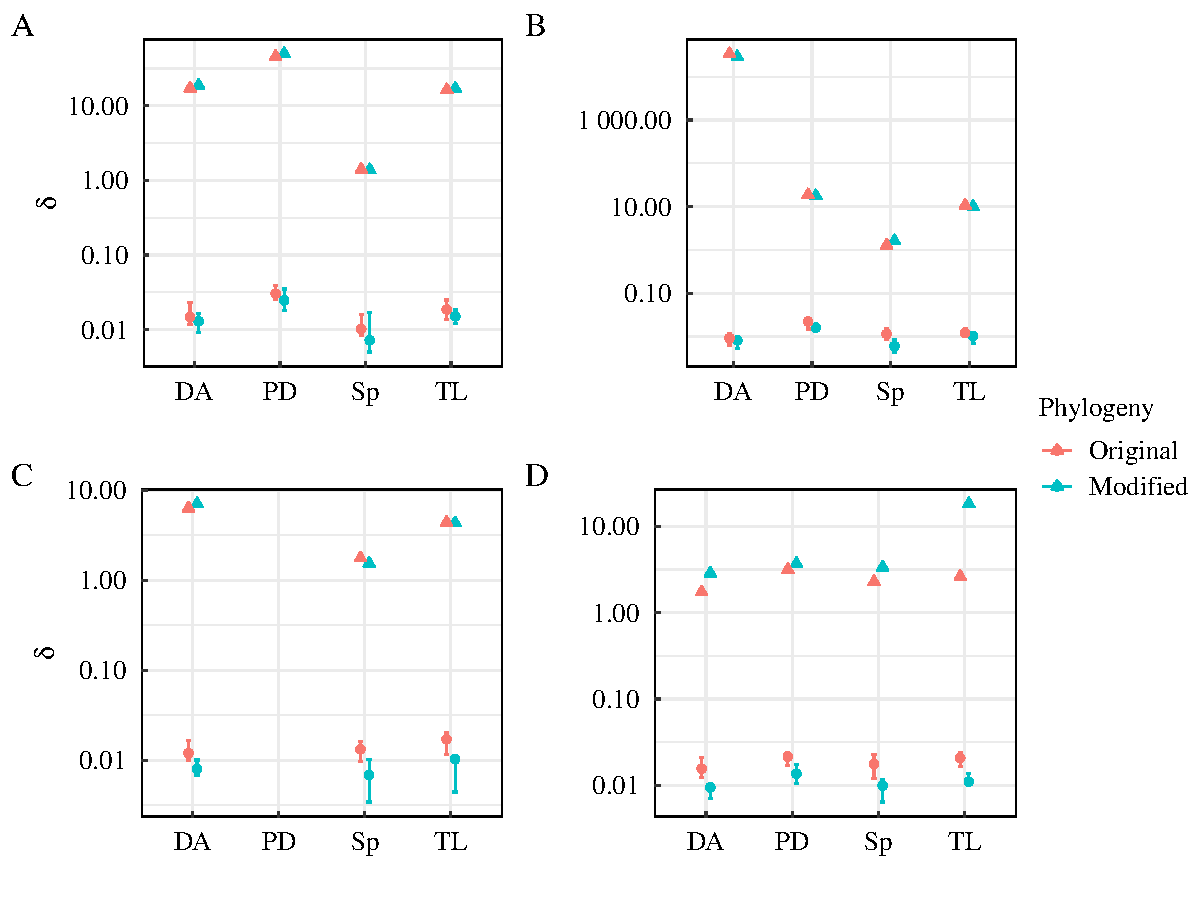
\includegraphics[scale=0.7]{figures/chapter2/Phylosignal/Categorical}
\caption[Phylogenetic signal in categorical traits ($\delta$) estimated with both original phylogenies and modified phylogenies]{\textbf{Phylogenetic signal in categorical traits ($\delta$) estimated with both original phylogenies and modified phylogenies.} \textbf{(A)} Mammals; \textbf{(B)} birds; \textbf{(C)} reptiles and \textbf{(D)} amphibians. Triangle-shaped points represent the estimated phylogenetic signal in each trait; round-shaped points represent the median null expectation of the phylogenetic signal ($\pm95\%CI$). Alterations of the phylogenies did not strongly impact $\delta$.}
\label{signalcategorical}
\end{figure}

\subsubsection{Missing trait values: imputation implementation}
Despite much variation in trait coverage across classes (see Results), results indicated strong phylogenetic signal in many categorical and continuous traits (Table \ref{physignal}).
I hence imputed missing trait values using random forest algorithms, implemented by missForest. As stated above, missForest was shown by Penone et al (2014) to be the best method when including phylogenetic information for mixed-type variable imputations. Phylogenetic relationships were included as additional predictors in the form of phylogenetic eigenvectors (Diniz-Filho 2012), extracted from the phylogenies using the PVR package (Santos 2018). Phylogenetic eigenvectors are computed from a phylogenetic distance matrix, and calculated using principal coordinate analysis methods. They summarise the relationships among species, and the first set of eigenvectors reflect larger distances, capturing divergences closer to the root (Diniz-Filho 2012). Penone et al (2014) showed that including the first 10 eigenvectors minimised the imputation error when imputing missing trait values with missForest. As such, I included the first 10 eigenvectors as additional predictors of missing trait values.   

As not all species were represented in the phylogenies (Figure \ref{species_rep_phylo}), I also added taxonomic orders as an extra predictor variable in the random forest algorithm. All traits in Table \ref{datasources} were included in the imputations (except for primary diet and diet breadth in reptiles). Tuning parameters of missForest were set to 10 maximum iterations (if the stopping criterion was not met beforehand, see below) and to 100 trees grown in each forests. To further examine imputation robustness and error, I imputed eight datasets in parallel (eight imputed trait datasets for each class).

\subsubsection{Imputation error and robustness}

\paragraph{Out-of-bag imputation error.}
To assess imputation accuracy, I used the `out-of-bag' error (OOB error) returned by the missForest function. The missForest algorithm proceeds iteratively, training random forests on observed values first, then predicting missing values over several iterations. When the difference between the last imputed dataset and the previous imputed dataset increases, the stopping criterion is met. The penultimate imputed dataset is then returned. For continuous variables, this difference, $\Delta_{cont}$,  is defined as:
\begin{align}
\Delta_{cont}=\frac{\sum_{j \in N}\left(X^{i,l}-X^{i,p}\right)^2}{\sum_{j \in N}\left(X^{i,l}\right)^2}, 
\end{align}
where $j$ is a continuous trait among $N$ traits, $X^{i,l}$ is the last imputed dataset and $X^{i,p}$ is the penultimate imputed dataset.  $\Delta_{cont}$ is a measure of the aggregated distance between two successive imputations across all continuous traits.  For categorical variables, the difference $\Delta_{cat}$ is:
\begin{align}
\Delta_{cat}=\frac{\sum_{k \in F}\sum_{j} J_{X^{i,l}\neq X^{i,p}}}{n(NA)}, 
\label{eqPFC}
\end{align}
where $k$ is a categorical trait among $F$ categorical traits, $n(NA)$ is a the number of missing values for $k$ and $J$ is the $j^{th}$ imputed values for which the consecutive imputations predicted contradicting results. In other words, $\Delta_{cat}$ measures the proportion of values that were found to be different between two successive imputations
(see Stekhoven (2011) for more details).

When the stopping criterion has been met, out-of-bag imputation errors can be estimated.
Out-of-bag errors refer to errors estimated from sub-samples of the data (bootstrap datasets, on which models are trained). Out-of-bag errors are estimated from these bootstrap datasets and as such differ from `true' imputation errors, which require previous knowledge of the full dataset. The true root-mean square error (root-MSE) for continuous traits is defined as: 
\begin{align}
\sqrt{\frac{mean\left(\left(X_t-X_i\right)^2\right)}{var\left(X_t\right)}}, 
\end{align}
where $X_t$ is a vector of the complete trait values and $X_i$ a vector of the imputed trait values (Stekhoven 2011). In case of an out-of-bag error, when the complete trait data is not provided, the MSE is calculated from the bootstrap datasets. For categorical traits, the out-of-bag PFC is calculated as the PFC ($\Delta_{cat}$, Equation \ref{eqPFC}), using the bootstrap sub-samples. Breiman (1996) showed that OOB estimates provide accurate estimations of the true imputation error. 

I retrieved OOB imputation errors (root-MSE and PFC) across eight imputed trait datasets in each class. I plotted the mean root-MSE and the mean PFC across the imputed datasets, as well as the range in errors (maximum error values and minimum errors values across all imputed datasets).

\paragraph{Imputation congruence.} To further assess whether imputations were robust, I investigated whether similar values were imputed across the eight datasets in each class, or in other words, whether results were congruent across the imputed datasets.  My expectation was that, for a trait, values imputed independently in different rounds should be nearly identical if imputations were robust. As such, for a continuous trait, pairwise correlations coefficients should be high across the eight datasets (correlation coefficients for the same trait imputed in pairwise independent rounds, see Table \ref{pairwisecorr}). For categorical traits, the random forest should predict the same values across the eight datasets. 

\begin{table}[h!]
\renewcommand{\baselinestretch}{1}
\renewcommand{\arraystretch}{1.5}
\begin{center}\fontsize{9}{11}\selectfont
\caption[Conceptual design for examining imputation congruence for continuous traits]{\textbf{Conceptual design for examining imputation congruence for continuous traits.} For one trait, pairwise correlation coefficients across eight independent imputation rounds are expected to be high if imputation are robust. To assess imputation congruence across eight imputed datasets, pairwise correlation coefficients were averaged (and the spread assessed using the range).} 
\label{pairwisecorr}
 \begin{tabular}{c|c|c|c|}
\cline{2-4}
\multicolumn{1}{l|}{}                    & \textbf{Imputed 1} & \textbf{Imputed 2} & \textbf{Imputed n} \\ \hline
\multicolumn{1}{|c|}{\textbf{Imputed 1}} & 1                  & -                  & -                  \\ \hline
\multicolumn{1}{|c|}{\textbf{Imputed 2}} & corr(1,2)          & 1                  & -                  \\ \hline
\multicolumn{1}{|c|}{\textbf{Imputed n}} & corr(n,1)          & corr(n,2)          & 1                  \\ \hline
\end{tabular}
\end{center}
\end{table}


For continuous traits, I assessed imputation congruence across the eight imputed datasets by averaging pairwise Pearson's correlation coefficients and plotting the mean (and range) for each trait. For categorical traits, I assessed congruence by assessing the percentage of species for which all eight imputed values were similar.




\section{Results}

\subsection{Outputs}
I collected and imputed data for 10 traits across 11637 avian species, 5502 mammalian species, 10334 reptilian species and 6904 amphibian species. Datasets recording species accepted and synonymic binomial names are available alongside the trait data. 

\subsection{Biases in the availability of trait information: non randomness in coverage and completeness and patterns in missing trait values}

\subsubsection{Increases in coverage and completeness due to taxonomic corrections.} 
Figure \ref{traitcov} shows the trait coverage within each class and for each trait, before and after correcting for taxonomy. Figure \ref{traitcomp} shows the distribution of trait completeness before and after taxonomic corrections, as well as the median trait completeness for each class.
Across all classes, correcting for taxonomy increased trait coverage (Figure \ref{traitcov}). Nevertheless, the increase in coverage for reptiles was marginal, which may indicate that the procedure developed to extract and identify accepted names overall performed less well for reptilian species than for mammals, birds and amphibians. Similarly, correcting for taxonomy improved trait completeness in all classes (Figure \ref{traitcomp}). Wilcoxon rank sum tests, testing the null hypothesis that uncorrected and corrected completeness distributions came from the same population, rejected this hypothesis across all classes (alternative hypothesis: uncorrected medians were lower than corrected medians; mammals: p-value=1.2$\cdot10^{-9}$; birds: p-value<2.2$\cdot10^{-16}$; reptiles: p-value=0.025; amphibians: p-value<2.2$\cdot10^{-16}$). To conclude, correcting for taxonomy had a significant impact on trait completeness and increased coverage in most cases. 

\subsubsection{Among-class biases in the availability of trait information}

\paragraph{Trait coverage.}
Trait coverage was highly variable across classes and traits. Trait coverage was initially good for most mammalian and avian traits, which had more than 50\% coverage (Figure \ref{traitcov} A and B). Only longevity had a coverage lower than 50\% for these classes, although generation length was above 80\% in both cases. Conversely, trait coverage was overall much poorer for reptiles and amphibians (Figure \ref{traitcov} C and D). About two-thirds of amphibian and reptilian traits presented a coverage below 50\%.  Amphibians and reptiles appeared to be less sampled in all traits, except in body mass (reptiles) and in body length, range size and habitat variables (amphibians).  As such, contrasting patterns of trait coverage appeared between, on the one hand, mammals and birds, and on the other hand, amphibians and reptiles. For species found in PREDICTS only, coverage increased disproportionally in reptiles and amphibians compared to the coverage for the full set of species (the figure for PREDICTS species only is available in the SI).

\begin{figure}[h!]
\centering
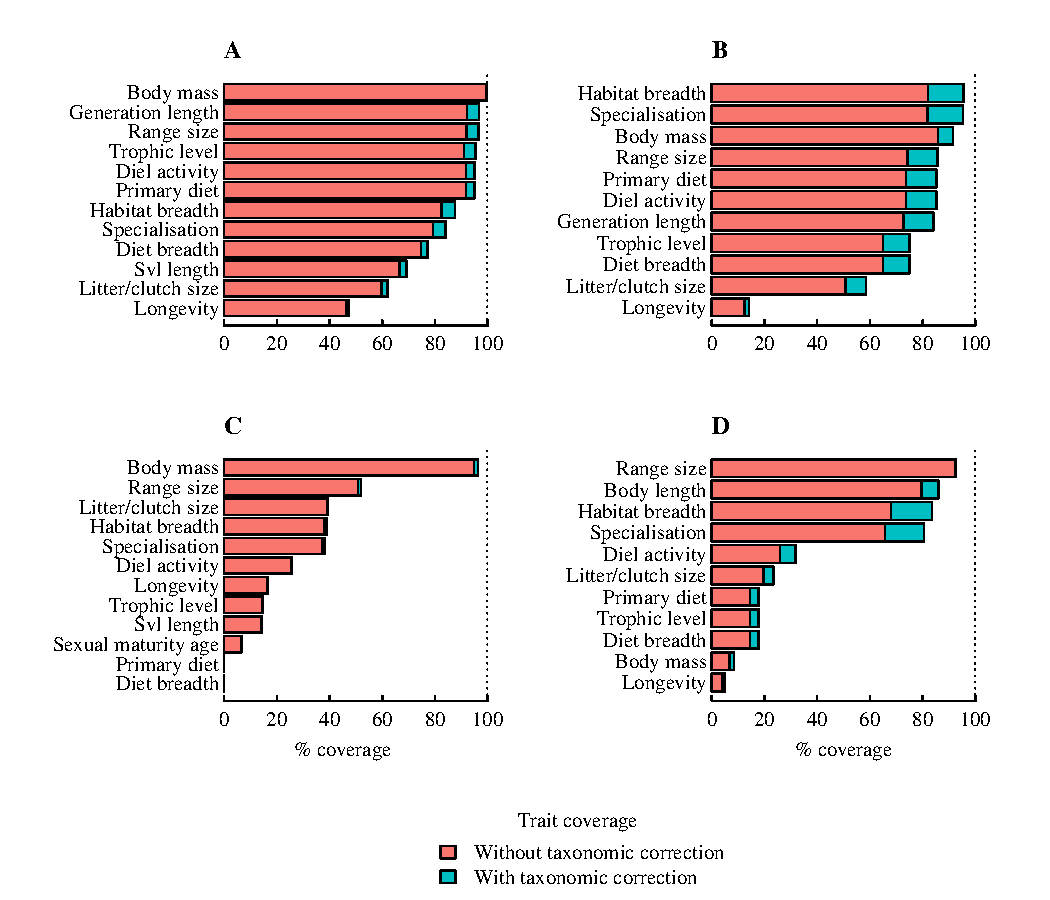
\includegraphics[scale=0.85]{figures/chapter2/Trait_coverage/Predictor_traits/All_species}
\caption[Trait coverage across all species before and after taxonomic correction]{\textbf{Trait coverage across all species before and after taxonomic correction.} Here are shown all targeted traits as well as a few other traits used in imputations, as additional predictors (such as generation length for mammals and birds or body length for amphibians). \textbf{(A)} Mammals (5885 species before correction, 5502 and after correction); \textbf{(B)} birds (13554 species before correction, 11637 after correction); \textbf{(C)} reptiles (10722 species before correction, 10334 after correction) and \textbf{(D)}; coverage across amphibians (8643 species before correction, 6904 after correction). Trait coverage was calculated as the percentage of species for which trait information was available. Correcting for taxonomic synonymy improved coverage in most cases. For mammals and birds, all traits had an initial coverage of more than 50\%, except longevity (but generation lengths were estimated for most species). On the other hand, trait coverage was poor (below 50\%) for about two thirds of collected reptilian and amphibian traits. A clear contrast in trait information appeared between mammals and birds versus amphibians and reptiles, highlighting the existence of important taxonomic biases in data collection.}
\label{traitcov}
\end{figure}

\paragraph{Trait completeness.}
Trait coverage revealed taxonomic biases, with higher resolution of trait information across mammals and birds. Trait completeness reflected similar biases. (Figure \ref{traitcomp}). The median completeness with taxonomic correction was high for mammals and birds (92\% and 82\% respectively) but much lower for reptiles and amphibians (30\% and 36\% respectively). A pairwise Kruskall-Wallis rank sum test rejected the hypothesis that completeness distribution across classes originated from the same distribution (p-values<2$\cdot10^{-16}$ in all cases), showing that class had a significant effect on the availability of trait information. 

\begin{figure}[h!]
\centering
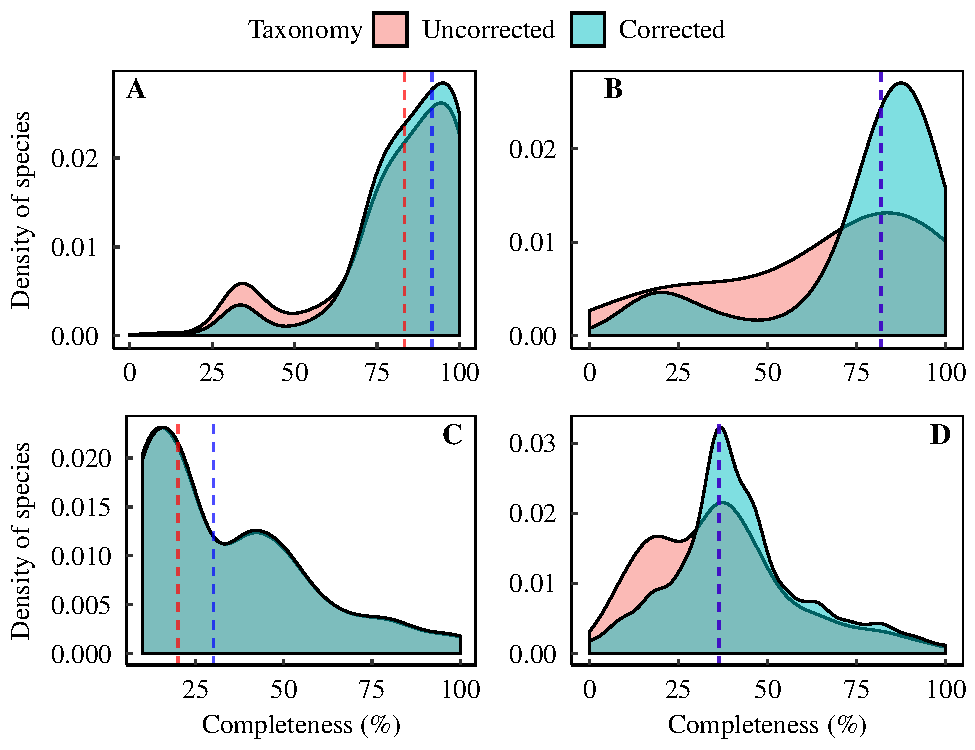
\includegraphics[scale=0.70]{figures/chapter2/Trait_coverage/Missing_values/Traitcompleteness}
\caption[Distribution of completeness of trait information across species]{\textbf{Distribution of completeness of trait information across species.} \textbf{(A)} Mammals; \textbf{(B)} birds; \textbf{(C)} reptiles and \textbf{(D)} amphibians. Completeness was calculated here for the same set of traits shown in Figure \ref{traitcov} (all predictor traits). Correcting for taxonomy affected completeness, significantly shifting the distributions to the right (alternative hypothesis, Wilcoxon rank sum tests: uncorrected medians were lower than corrected medians; mammals: p-value=1.2$\cdot10^{-9}$; birds: p-value<2.2$\cdot10^{-16}$; reptiles: p-value=0.025; amphibians: p-value<2.2$\cdot10^{-16}$). Class had a significant effect on median trait completeness (a pairwise Kruskall-Wallis rank sum test rejected the null hypothesis that completeness distributions across classes originated from the same distribution (p-values<$2\cdot10^{-16}$ in all cases)).}
\label{traitcomp}
\end{figure}

\subsubsection{Non-randomness in trait information availability within classes: patterns of missing trait values with regards to phylogenies}
Beyond cross-class biases in the availability of trait information, within-class patterns of missing values were revealed when plotting within-family median completeness and coverage against phylogenetic trees built at the family level.

\paragraph{Within-class patterns of trait completeness.}
Figure \ref{classcomp} shows within-family trait completeness for each class, colour-coded in the tree branches. For better visualisation, the trees are represented without tip labels. Figures providing tip labels are available in the SI (for each class, tip label information includes taxonomic order and family). As expected from the distribution of completeness values for mammals and birds, within-family completeness was high across most branches of the trees. In mammals, Chiropteras appeared to have lower median trait completeness than other orders (light blue cluster appearing in the middle of the tree, Figure \ref{classcomp}A). In birds, no particular structure seemed to emerge in within-family median completeness (although the upper part of the phylogeny, corresponding to Procellariiformes, Charadriiformes, and Anseriformes appeared to be particularly well sampled, Figure \ref{classcomp}B). In herptiles, nevertheless, clusters of similar completeness appeared at family levels. For reptiles, the lower part of the tree appeared to be particularly less well sampled than the above part of the tree (encompassing families such as Tropidophiidae, Lamprophiida or Typhlopidae: mostly, snakes; \ref{classcomp}C). In amphibians, families in the Anura order showed both the best and worst median completeness (Figure \ref{classcomp}D). 

\begin{figure}[h!]
\centering
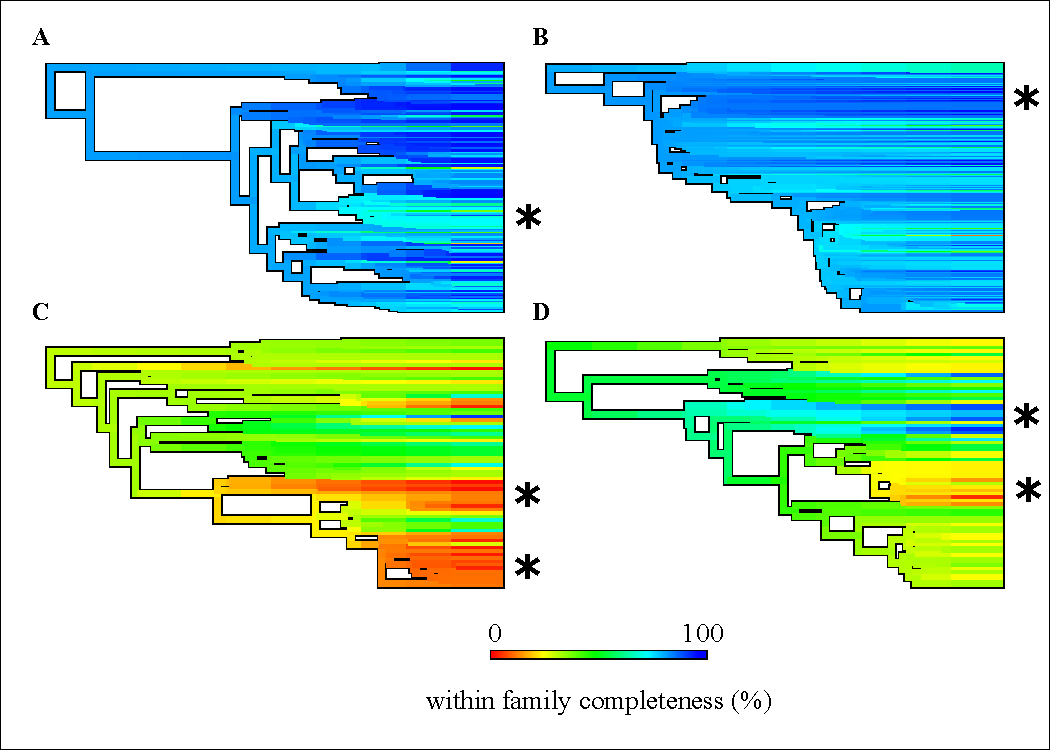
\includegraphics[scale=0.75]{figures/chapter2/NA_phylo_patterns/Completeness_all}
\caption[Median completeness across families]{\textbf{Median completeness across families.} Tips labels are not shown here for better visualisation of the results; the same figures with tip labels are provided in the SI (zooming into the figure is necessary for mammals and birds); tip label information includes order and family. \textbf{(A)} Mammalian family tree; \textbf{(B)} avian family tree; \textbf{(C)} reptilian family tree and \textbf{(D)} amphibian family tree. Median trait completeness was calculated within families and colour-coded  against tree branches. Family clusters of similar median trait completeness appear, particularly in reptile and amphibians.}
\label{classcomp}
\end{figure}

Overall, these results showed that trait completeness was not random with regards to the phylogenetic relatedness of families. Closely related families seemed to share more similar median trait completeness than less closely related families. As such, the availability of trait information for a species may be dependent on its phylogenetic history; many other factors may interplay with species evolutionary history to explain these patterns. 

\paragraph{Within-class patterns of trait coverage.} Figures \ref{familycov_mammals}, \ref{familycov_birds}, \ref{familycov_reptiles} and \ref{familycov_amphibians} show within-family median trait coverage. In each figure, the subplots are ordered from the trait showing highest overall coverage to the trait showing lowest overall coverage (as in Figure \ref{traitcov}. In each figure, the last subplot represents the contribution of each family to the total number of species in the phylogeny. 

Overall, these plots showed that for each trait, phylogenies seemed to be sampled non-randomly, with apparent clusters more visible as trait coverage decreased. Moreover, which families were better sampled was not 

\pagebreak

% Mammals
\begin{figure}[h!]
\centering
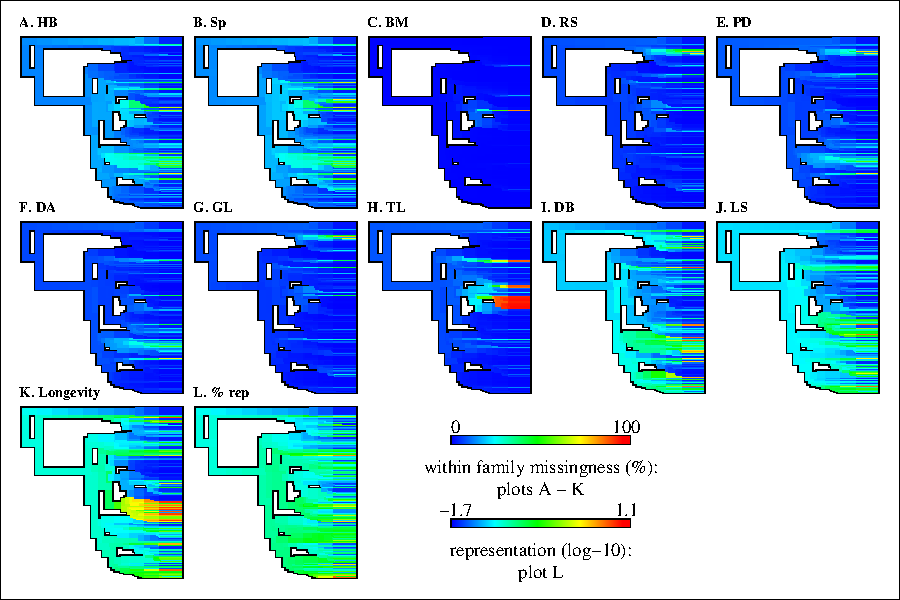
\includegraphics[scale=1]{figures/chapter2/NA_phylo_patterns/Mammals_coverage}
\caption[Within-family trait coverage in mammals]{\textbf{Within-family trait coverage in mammals.}}
\label{familycov_mammals}
\end{figure}

% Birds
\begin{figure}[h!]
\centering
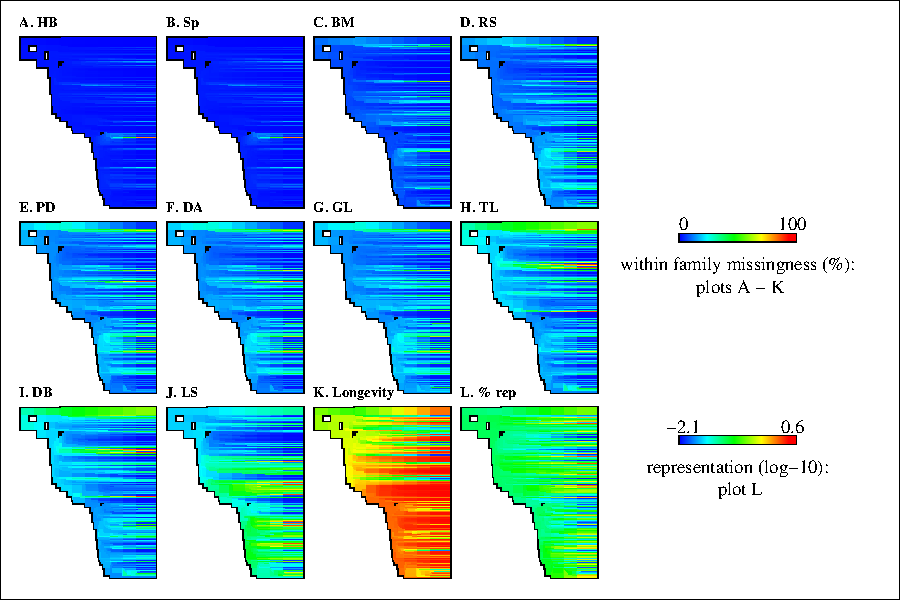
\includegraphics[scale=1]{figures/chapter2/NA_phylo_patterns/Birds_coverage}
\caption[Within-family trait coverage in birds]{\textbf{Within-family trait coverage in birds.}}
\label{familycov_birds}
\end{figure}

\pagebreak

% Reptiles
\begin{figure}[h!]
\centering
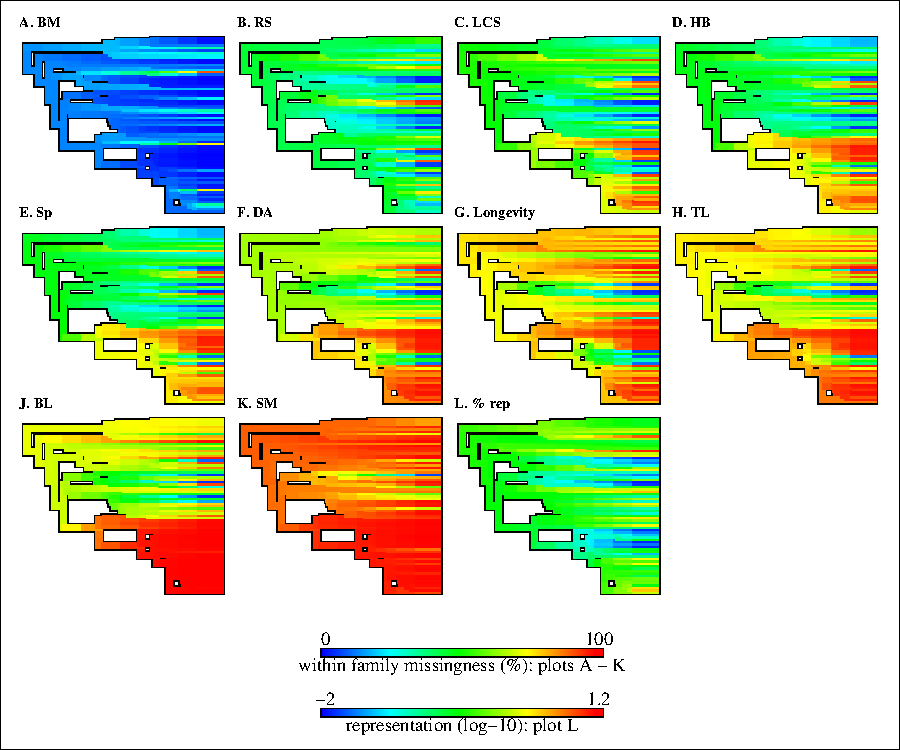
\includegraphics[scale=1]{figures/chapter2/NA_phylo_patterns/Reptiles_coverage}
\caption[Within-family trait coverage in reptiles (squamates)]{\textbf{Within-family trait coverage in reptiles (squamates).}}
\label{familycov_reptiles}
\end{figure}

% Amphibians
\begin{figure}[h!]
\centering
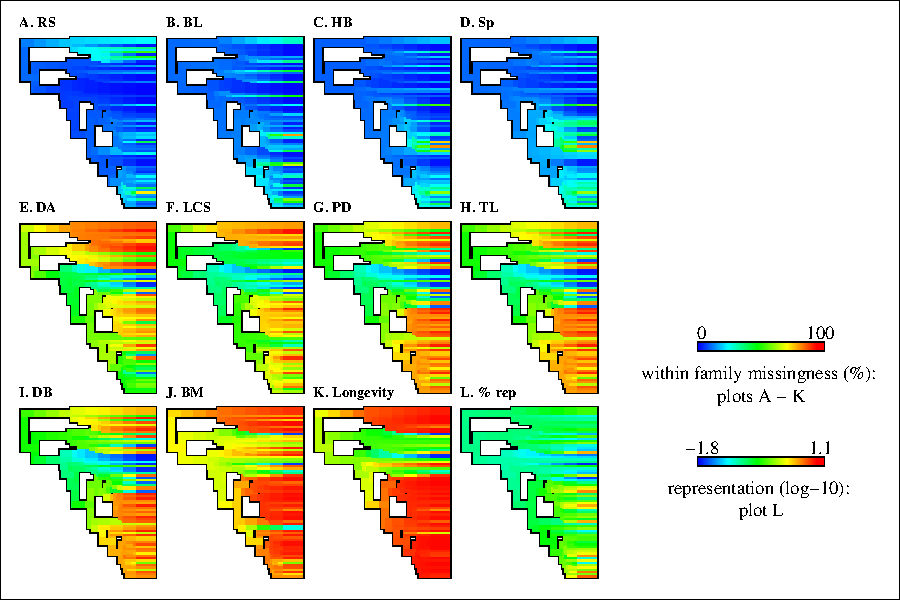
\includegraphics[scale=1]{figures/chapter2/NA_phylo_patterns/Amphibians_coverage}
\caption[Within-family trait coverage in amphibians]{\textbf{Within-family trait coverage in amphibians.}}
\label{familycov_amphibians}
\end{figure}



\pagebreak
\subsection{Imputation performance and robustness}

\subsubsection{Out-of-bag imputation errors}
Figure \ref{OOBerrors}A shows out-of-bag root-mean-squared errors for each continuous traits (shown here for one randomly selected imputed dataset). Figure \ref{OOBerrors}B is the out-of-bag proportion of falsely classified values for categorical for the same imputed dataset.
Estimated prediction errors for categorical traits were low to moderate (all below XX \%). For continuous traits, estimated errors could be large (e.g., mammalian body mass, amphibian clutch size  or range sizes). Nevertheless, such large errors were driven by high trait values in the dataset. Figure \ref{traitdist} shows the distribution of trait values after imputations; large prediction errors are estimated where traits can attain high values. 
 
\begin{figure}[h!]
\centering
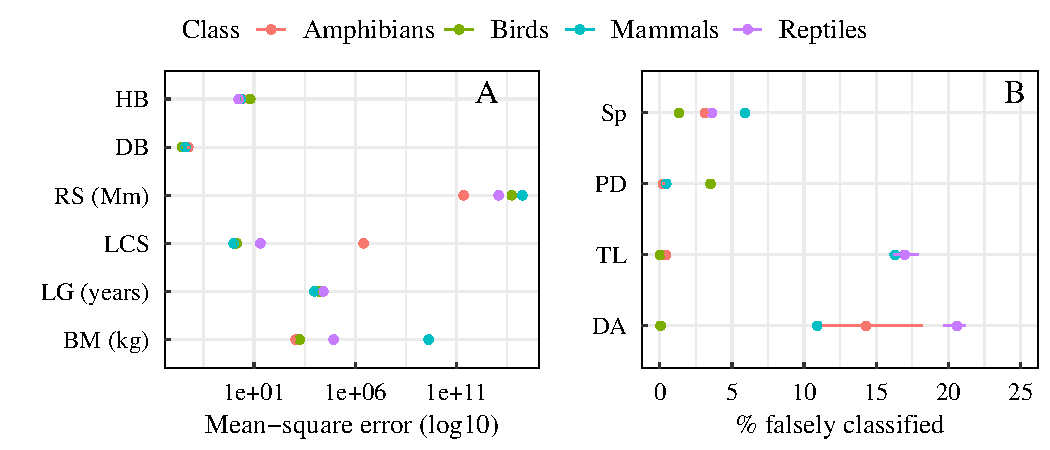
\includegraphics[scale=0.75]{figures/chapter2/Imputation_errors/MSE_PFC}
\caption[missForest out-of-bag root-mean-square errors and proportion of falsely classified values]{\textbf{missForest out-of-bag root-mean-squared errors and proportion of falsely classified values.} \textbf{(A)} Out-of-bag root-mean-square errors for continuous traits. \textbf{(B)} Out-of-bag proportion of falsely classified values.}
\label{OOBerrors}
\end{figure}

\begin{figure}[h!]
\centering
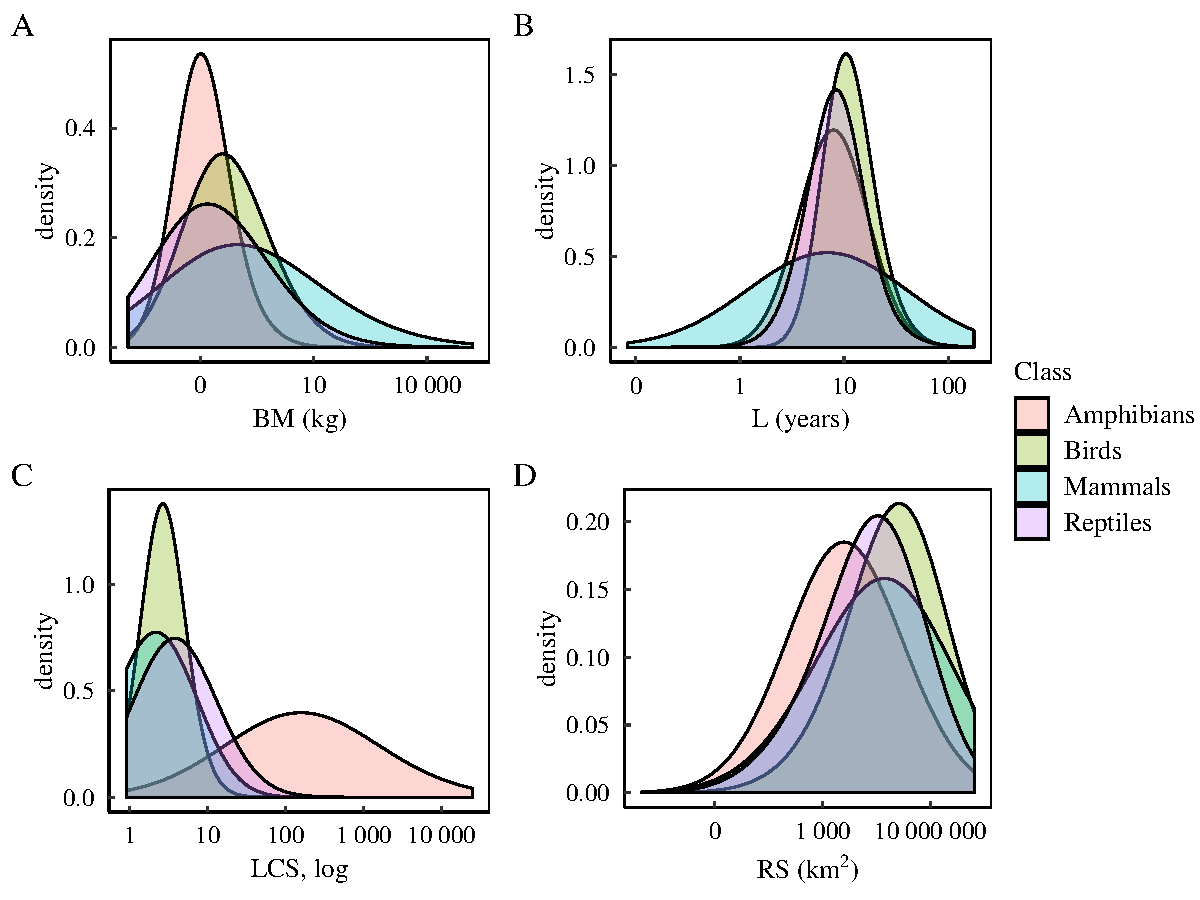
\includegraphics[scale=0.7]{figures/chapter2/Imputation_errors/Distributions}
\caption[Distribution of trait values after imputation for body mass, longevity, litter/clutch size and distribution of range sizes]{\textbf{Distribution of trait values after imputation for body mass, longevity, litter/clutch size and distribution of range sizes.}}
\label{traitdist}
\end{figure}



\subsubsection{Congruence of imputed values among eight imputed datasets}

Figure \ref{congruence}A shows the range and mean of pairwise correlation coefficients obtained for each trait, across eight imputed datasets. Pairwise correlation coefficients were calculated for each trait, predicted in eight independent imputation rounds, so that high correlation  values indicated more similar predictions for one trait across the eight datasets. Overall, imputation congruence was high for all continuous traits except habitat breadth. Imputation congruence was high across all classes for longevity (minimum mean correlation coefficient of 0.87 for reptiles), but more variable in other traits depending on the class.
Figure \ref{congruence}B shows the proportion of species for which imputed values were similar across the eight imputed datasets. At least 50\% of all species had similar predicted values across all imputed traits. Imputation congruence was high for trophic level (above 86\% in all classes), and more variable in other traits depending on the class. 

Mammals had the best imputation congruence scores in both continuous and categorical traits (minimum mean correlation coefficient of 0.85 for continuous traits and minimum percentage of agreement of 85\% for categorical traits). Imputation congruence for birds was also very good, though scores were slightly lower for diet related variables (diet breadth and primary diet). For amphibians and reptiles, mean correlation coefficients were all above 0.60, except for habitat breadth. For amphibians in particular, imputation congruence on habitat breadth was poor. Overall, imputed results for amphibians were less congruent than for reptiles, birds and mammals.

\begin{figure}[h!]
\centering
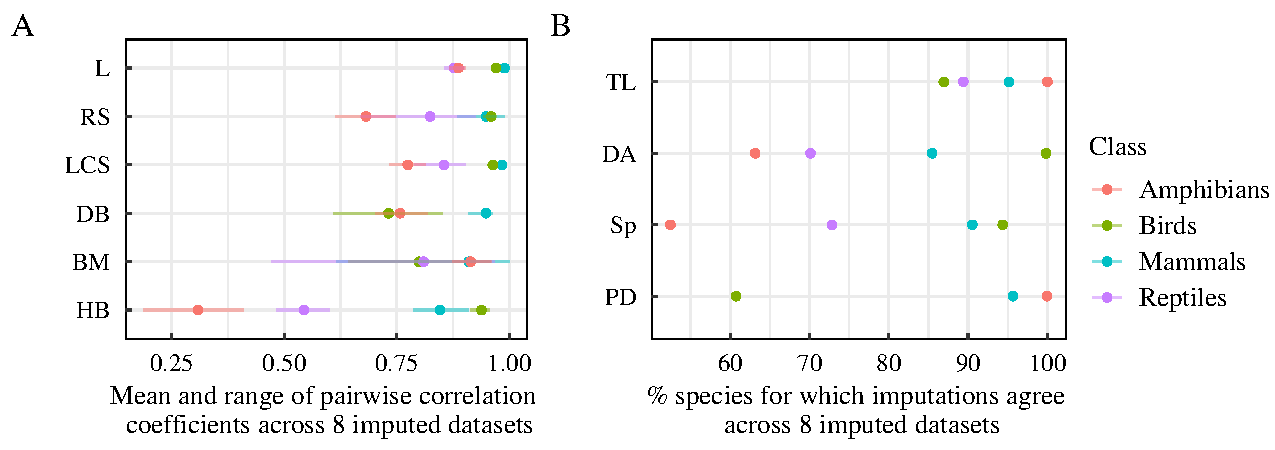
\includegraphics[scale=0.75]{figures/chapter2/Congruence_imputations/Summary}
\caption[Imputation congruence across eight imputed datasets]{\textbf{Imputation congruence across eight imputed datasets.}}
\label{congruence}
\end{figure}


\pagebreak
\section{Discussion}

% biases
% imputation robustness and error

In this work, I compiled and imputed data on 10 traits across x mammalian, x reptilian, x avian and x amphibian species. Traits related to species morphological characteristics (body mass), to their life-history (litter/clutch size, longevity, diel activity, ), to their habitat preferences (habitat breadth, specialisation), and to their diet (trophic level; for mammals, birds and amphibians only, primary diet and diet breadth were also collated). To my knowledge, there is yet no published or freely available trait database encompassing all terrestrial vertebrates. As such, this work could constitute one of the first attempts to collate extensive trait information across all terrestrial vertebrates, enabled by all past and recent efforts to release trait information in the public domain.

Further developments could include enhancing the existing data to improve initial trait coverage. Alternatively, if novel primary sources were released, new variables could be added; even though the traits included in this work already encompass most of the ecological traits available in the literature across vertebrate classes, one notable omission was species mobility. Species abilites to both move within their habitats (home range) and to disperse and colonise new areas is likely to have a major impact on their aptitudes to cope with anthropogenic changes. Nevertheless, traits relating to mobility in amphibians or reptiles were unavailable. Relating to species movement, the only readily available variable that could have been added was volancy, assuming that most amphibians and reptiles were non-volant. Other  information that could further enhance the dataset include reptilian diet, foraging strata and terrestriality (species habitat preferences along a vertical gradient: e.g. above versus below ground prefences). Note that the current compiled and imputed dataset contains fossil species, as some of the primary sources provided estimates for these. Such species could be filtered out in the future.

This works highlighted several frequent issues met when working with a large number of species or when working with dasasets from different origins. For categorical variables, the levels of the least resolved dataset had to be adopted across all classes, even though more detailed information was avaible in another class. Indeed, common denominators had to be found, at the expanse of highly resolved data. One example was diel activity time, that I had to constrain to two categories (nocturnal or non-nocturnal). The main reason for this was that most primary sources focused on one class only, while only a few encompassed more than two classes. Similarly, I did not compile any metric reflecting intra-specific variability in continuous traits. Intra-specific variability has been shown to have important effects on ecological systems, and a growing body of literature encourages trait-based research to include intraspecific variability in research studies. Here, metrics reflecting intraspecific variability were excluded due to both the scale of the data compilation and the lack of estimates across classes.

One major issue in this work was the taxonomic `pseudoreplication' of species due to the presence of similar species under diverse names, and other taxonomic errors. To a lesser extent, where older taxonomic classification systems were used, inaccurate order or family information was provided in the primary sources. Taxonomic errors and replication of names are a major issue in ecology. This issue, which has been termed `taxonomic inflation', is difficult to tackle at large scales (Isaac et al 2004). The lack of a comprehensive and universal database for species names complicates species identification, as well as unresolved taxonomy and taxonomic revisions (for example, one species being split into two subspecies, or the opposite).
Taxonomic synonymy and taxonomic errors in general have been found to be a severe issue in diversity studies; for example, they can impediment accurate estimations of species number (Cardoso 2017). In this work, I showed that taxonomic synonymy artificially increased the amount of missing trait values by creating pseudoreplicates of the same species, also inflating the overall number of species and significantly lowering median trait completeness. The procedure that I developed to tackle taxonomic redundancy was itself highly dependent on the quality of the taxonomic information in the Red List and the ITIS. Overall, the procedure was not optimal, and a number of issues could be addressed to try and improved it. Nevertheless, it participated in reducing taxonomic mismatches and in increasing the number of matches across datasets. Some initiative, such as the Taxonomic Name Resolution Service for plants (http://tnrs.iplantcollaborative.org/) attempt to tackle taxonomic inflation by providing a free tool to standardise plant names and retrieve current accepted names. Up to five thousand species names can be submitted at once. The Global Information System provides a similar tool, which nevertheless does not systematically return species accepted names (but their status and a confidence level), and is as such less practical. Nonetheless, such databases are an invaluable source of information and should encourage researchers to try and standardise taxonomy.

% biases in trait information

In October 2018, Cooke et al released a dataset of six mammalian and avian trait. The methods they used to compile and impute trait data were very similar to the methods used in this work. The most notable divergences were the use of different imputation methods (multivariate chained equations) and the pre-selection of traits with more than 50\% coverage in Cooke et al. Because very similar primary sources were used, I did not directly use their data in my work. Nevertheless, I compared the results of both data collection and imputation (see SI). 
Using non parametric random forest algorithms, as implemented in R by the missForest function, presented several advantages over other imputation methods. First, random forests could deal with mixed type variables, and estimate out-of-bag errors for each variable. Second, no underlying data distribution was assumed in the process, as it builds upon non-parametric processes. Third, missForest was computationally faster than other functions, which was an important criterion. Morever, missForest was found to be the best available method to use when imputing trait data with phylogenetic information. Nevertheless, even though missForest was found to be robust to missing values, no study has investigated imputations robustness with an amount of missing values as big as it was here. Moreover clustering of missing trait values in the phylogeny.

Despite these advantages, the robustness to imputations needs to be investigated further, for reasons that I detail below.


\paragraph{Conclusion}

I presented in this Chapter  

The methods for compiling trait data may be revisited in the future, and the trait data is likely to be enhanced or to slightly change if imputed again.

Future work will build upon the trait data collated as described in this chapter. I illustrate the first use of this data with the next chapter, which investigates how land-use change impacts the functional diversity of vertebrate communities. In the last chapter, I detail some research questions that this data will allow to investigate in the future months on my PhD.


Completeness is likely to have an important effect on trait imputations, as it is a reflection of how many predictors have an estimate for a species.